\chapter{Specifikacija programske potpore}

\section{Funkcionalni zahtjevi}			

\noindent \textbf{Dionici:}

\begin{packed_enum}
	
	\item Ovlašteni zaposlenik tvrtke
	\item Klijent
	\item Administrator
	\item Razvojni tim
	
\end{packed_enum}

\noindent \textbf{Aktori i njihovi funkcionalni zahtjevi:}


\begin{packed_enum}
	\item  \underbar{Neregistrirani/neprijavljeni korisnik (inicijator) može:}
	
	\begin{packed_enum}
		
		\item vidjeti kartu s parkiralištima (adresa, broj ukupnih i slobodnih mjesta, cijena)
		\item registrirati se i/ili prijaviti se (kao klijent ili tvrtka)
		
	\end{packed_enum}
	
	\item  \underbar{Klijent (inicijator) može:}
	
	\begin{packed_enum}
		
		\item vidjeti kartu s parkiralištima (adresa, broj ukupnih i slobodnih mjesta, cijena)
		\item pregledavati, uređivati i izbrisati korisnički račun
		\item pregledavati, uređivati i izbrisati vozila
		\item pregledavati, uređivati i izbrisati kartice
		\item rezervirati parkirališno mjesto
		\item pregledavati, uređivati i izbrisati rezervacije
		\item pisati i pregledavati  recenzije
		\item tražiti upute do parkirališta
		
	\end{packed_enum}
	
	
	\item  \underbar{Ovlašteni zaposlenik tvrtke (inicijator) može:}
	
	\begin{packed_enum}
		
		\item vidjeti kartu s parkiralištima
		\item pregledavati, uređivati, dodavati i brisati svoja parkirališta
		\item pregledavati, uređivati i izbrisati korisnički račun
		\item pregledavati vlastite i tuđe recenzije
		\item pregledavati rezervacije na vlastitim parkiralištima
		\item odgovoriti na recenzije korisnika
		
	\end{packed_enum}
	
	\item \underbar{Administrator (inicijator) može:}
	
	\begin{packed_enum}
		
		\item vidjeti popis svih registriranih korisnika i osnovnih podataka
		\item pregledavati rezervacije
		\item brisati i mijenjati razinu pristupa aplikaciji drugim korisnicima
		\item brisati recenzije
		\item dodavati ili brisati parkirališta
		
	\end{packed_enum}
	
	\item \underbar{Baza podataka (sudionik) može:}
	
	\begin{packed_enum}
		
		\item pohranjivati podatke o korisnicima (osobni podatci, kartica, vozila)
		\item pohranjivati podatke o parkiralištima (njihovim kapacitetima i ponudama)
		\item pohranjivati podatke o rezervacijama
		\item pohranjivati podatke o tvrtkama
		
	\end{packed_enum}
\end{packed_enum}


\eject 



\subsection{Obrasci uporabe}

\subsubsection{Opis obrazaca uporabe}


\newcounter{uccounter}
\newcommand\showuccounter{\stepcounter{uccounter}\theuccounter}


\noindent \underbar{\textbf{UC\showuccounter\ - Pregled karte}}
\begin{packed_item}
	
	\item \textbf{Glavni sudionik: } Korisnik
	\item \textbf{Cilj:} Pogledati kartu s označenim parkiralištima
	\item \textbf{Sudionici:} Baza podataka
	\item \textbf{Preduvjet:} -
	\item \textbf{Opis osnovnog tijeka:}
	
	\item[] \begin{packed_enum}
		
		\item Korisnik otvara aplikaciju
		\item Prikazuje se karta s označenim parkiralištima

	\end{packed_enum}
	
	\item[] \begin{packed_item}
	
		\item[1.a] Korisnik je već u aplikaciji
		\item[] \begin{packed_enum}
			
			\item Korisnik odabire pregled karte
			
	    \end{packed_enum}
    \end{packed_item}
\end{packed_item}

\noindent \underbar{\textbf{UC\showuccounter\ - Pregled podataka o parkiralištu na karti}}
\begin{packed_item}
	
	\item \textbf{Glavni sudionik:} Korisnik
	\item \textbf{Cilj:} Pregleda podataka o parkiralištu
	\item \textbf{Sudionici:} Baza podataka
	\item \textbf{Preduvjet:} Otvorena karta
	\item \textbf{Opis osnovnog tijeka:}
	
	\item[] \begin{packed_enum}
		
		\item Korisnik pritišće na oznaku parkirališta na karti
		\item Prikazuju se osnovni podatci o parkiralištu i o tvrtki koja je nadležna za to parkiralište

	\end{packed_enum}
\end{packed_item}

\noindent \underbar{\textbf{UC\showuccounter\ - Prijava korisnika}}
\begin{packed_item}

	\item \textbf{Glavni sudionik:} Korisnik
	\item \textbf{Cilj:} Prijaviti korisnika
	\item \textbf{Sudionici:} Baza podataka
	\item \textbf{Preduvjet:} Korisnik nije prijavljen
	\item \textbf{Opis osnovnog tijeka:}
	
	\item[] \begin{packed_enum}
		
		\item Korisnik odabire opciju za prijavu korisnika
		\item Otvara se forma za popunjavanje korisničkih podataka potrebnih za prijavu
		\item Korisnik je prijavljen u aplikaciju i preusmjeren na početni zaslon aplikacije

	\end{packed_enum}

	\item  \textbf{Opis mogućih odstupanja:}
	
	\item[] \begin{packed_item}
	
		\item[2.a] Nevažeći podaci prilikom prijave korisnika
		\item[] \begin{packed_enum}
			
			\item Korisniku se prikazuje poruka o nevažećim podacima
			\item Korisnik ispravlja nevažeće podatke za prijavu ili odustaje od prijave
			
		\end{packed_enum}
		
		\item[2.b] Korisnik je zaboravio lozinku za prijavu
		\item[] \begin{packed_enum}
			
			\item Prikazuje se poruka o pogrešnim podacima za prijavu 
			\item Korisnik odabire akciju za ponovno postavljanje lozinke
			\item Otvara se forma za unos emaila
			\item Na email adresu mu se šalje poveznica koja ga vodi na formu za postavljanje nove lozinke te ju korisnik popunjava
			\item Lozinka je promijenjena
			\item Korisnik se preusmjerava na formu za prijavu
			
		\end{packed_enum}

	\end{packed_item}
\end{packed_item}

\noindent \underbar{\textbf{UC\showuccounter\ - Registracija korisnika}}
\begin{packed_item}

	\item \textbf{Glavni sudionik:} Korisnik
	\item \textbf{Cilj:} Registrirati korisnika
	\item \textbf{Sudionici:} Baza podataka
	\item \textbf{Preduvjet:} Korisnik nije prijavljen niti registriran
	\item \textbf{Opis osnovnog tijeka:}
	
	\item[] \begin{packed_enum}
		
		\item Korisnik odabire opciju za registraciju korisnika
		\item Otvara se forma za popunjavanje korisničkih podataka
		\item Korisnik otvara novi račun i prikazuje mu se poruka da je račun uspješno stvoren
		\item Korisnik je automatski prijavljen u sustav

	\end{packed_enum}

	\item  \textbf{Opis mogućih odstupanja:}
	
	\item[] \begin{packed_item}
	
		\item[3.a] Nevažeći podatci prilikom registracije korisnika
		\item[] \begin{packed_enum}
			
			\item Korisnik se obavještava o neuspjeloj registraciji
			\item Korisnik ispravlja nevažeće podatke te pokušava ponovno ili odustaje od registracije
			
		\end{packed_enum}
		
	\end{packed_item}
\end{packed_item}

\noindent \underbar{\textbf{UC\showuccounter\ - Pregled podataka o korisničkom računu}}
\begin{packed_item}
	
	\item \textbf{Glavni sudionik:} Korisnik
	\item \textbf{Cilj:} Pregledati podatke o korisničkom računu
	\item \textbf{Sudionici:} Baza podataka
	\item \textbf{Preduvjet:} Korisnik je prijavljen
	\item \textbf{Opis osnovnog tijeka:}
	
	\item[] \begin{packed_enum}
		
		\item Korisnik otvara podatke o korisničkom računu
		\item Prikažu se podatci o korisničkom računu
	
	\end{packed_enum}
	
\end{packed_item}

\noindent \underbar{\textbf{UC\showuccounter\ - Uređivanje podataka o korisničkom računu}}
\begin{packed_item}
	
	\item \textbf{Glavni sudionik:} Klijent/Tvrtka
	\item  \textbf{Cilj:} Urediti podatke o korisničkom računu
	\item  \textbf{Sudionici:} Baza podataka
	\item  \textbf{Preduvjet:} Administrator/Tvrtka je prijavljen
	\item  \textbf{Opis osnovnog tijeka:}
	
	\item[] \begin{packed_enum}
		
		\item Korisnik otvara podatke o korisničkom računu
		\item Prikažu se podatci o korisničkom računu
		\item Korisnik odabire akciju za uređivanje
		\item Prikaže se forma za uređivanje podataka o korisničkom računu
		\item Korisnik uređuje podatke
		\item Korisnik sprema promjene
	
	\end{packed_enum}
	
	\item  \textbf{Opis mogućih odstupanja:}
	
	\item[] \begin{packed_item}
		
		\item[6.a] Nevažeći podatci prilikom spremanja promjena
		\item[] \begin{packed_enum}
			
			\item Korisniku se prikazuje poruka o nevažećim podacima
			\item Korisnik ispravlja podatke
			\item Korisnik ponovno sprema podatke
			
		\end{packed_enum}
		
	\end{packed_item}
\end{packed_item}

\noindent \underbar{\textbf{UC\showuccounter\ - Brisanje korisničkog računa}}
\begin{packed_item}
	
	\item \textbf{Glavni sudionik:} Korisnik
	\item  \textbf{Cilj:} Izbrisati korisnički račun
	\item  \textbf{Sudionici:} Baza podataka
	\item  \textbf{Preduvjet:} Korisnik je prijavljen
	\item  \textbf{Opis osnovnog tijeka:}
	
	\item[] \begin{packed_enum}
		
		\item Korisnik otvara podatke o svom računu
		\item Korisnik odabire akciju za brisanje računa
		\item Briše se korisnikov račun
		\item Korisnik se preusmjerava na početni zaslon
		
	\end{packed_enum}
\end{packed_item}

\noindent \underbar{\textbf{UC\showuccounter\ - Pregled podataka o vozilu}}
\begin{packed_item}
	
	\item \textbf{Glavni sudionik:} Klijent
	\item \textbf{Cilj:} Pregledati podatke o vozilu
	\item \textbf{Sudionici:} Baza podataka
	\item \textbf{Preduvjet:} Klijent je prijavljen
	\item \textbf{Opis osnovnog tijeka:}
	
	\item[] \begin{packed_enum}
		
		\item Klijent otvara popis vozila
		\item Klijent odabire parkiralište koje želi pregledati
		\item Prikažu se podaci o vozilu
	
	\end{packed_enum}
\end{packed_item}

\noindent \underbar{\textbf{UC\showuccounter\ - Dodavanje vozila}}
\begin{packed_item}

	\item \textbf{Glavni sudionik:} Klijent
	\item \textbf{Cilj:} Dodati vozilo
	\item \textbf{Sudionici:} Baza podataka
	\item \textbf{Preduvjet:} Klijent je prijavljen
	\item \textbf{Opis osnovnog tijeka:}
	
	\item[] \begin{packed_enum}
		
		\item Klijent otvara formu za dodavanje vozila
		\item Unose se svi potrebni podaci
		\item Klijent odabire akciju za dodavanje vozila
		\item Vozilo je dodano

	\end{packed_enum}
	
	\item  \textbf{Opis mogućih odstupanja:}
	
	\item[] \begin{packed_item}
		
		\item[6.a] Nevažeći podatci prilikom dodavanja vozila
		\item[] \begin{packed_enum}
			
			\item Klijentu se prikazuje poruka o nevažećim podacima
			\item Klijent ispravlja podatke
			\item Klijent ponovno odabire akciju za dodavanje vozila
			
		\end{packed_enum}
		
	\end{packed_item}
\end{packed_item}

\noindent \underbar{\textbf{UC\showuccounter\ - Uređivanje vozila}}
\begin{packed_item}
	
	\item \textbf{Glavni sudionik:} Klijent
	\item \textbf{Cilj:} Urediti podatke o vozilu
	\item \textbf{Sudionici:} Baza podataka
	\item \textbf{Preduvjet:} Klijent je prijavljen
	\item \textbf{Opis osnovnog tijeka:}
	
	\item[] \begin{packed_enum}
		
		\item Klijent otvara popis vozila
		\item Klijent odabire vozilo koje želi urediti
		\item Otvara se forma za uređivanje vozila popunjena sa podacima odabranoga vozila
		\item Klijent uređuje podatke
		\item Klijent sprema promjene
	
	\end{packed_enum}
	
	\item  \textbf{Opis mogućih odstupanja:}
	
	\item[] \begin{packed_item}
		
		\item[6.a] Nevažeći podatci prilikom spremanja promjena
		\item[] \begin{packed_enum}
			
			\item Klijentu se prikazuje poruka o nevažećim podacima
			\item Klijent ispravlja podatke
			\item Klijent ponovno sprema podatke
			
		\end{packed_enum}
		
	\end{packed_item}

\end{packed_item}

\noindent \underbar{\textbf{UC\showuccounter\ - Uklanjanje vozila}}
\begin{packed_item}
	
	\item \textbf{Glavni sudionik:} Klijent
	\item \textbf{Cilj:} Ukloniti vozilo
	\item \textbf{Sudionici:} Baza podataka
	\item \textbf{Preduvjet:} Klijent je prijavljen
	\item \textbf{Opis osnovnog tijeka:}
	
	\item[] \begin{packed_enum}
		
		\item Klijent otvara popis vozila
		\item Klijent odabire vozilo koje želi ukloniti
		\item Prikažu se detalji vozila
		\item Klijent odabire akciju uklanjanja vozila
		\item Klijent je preusmjeren na popis vozila

	\end{packed_enum}
\end{packed_item}

\noindent \underbar{\textbf{UC\showuccounter\ - Pregled podataka o parkiralištu}}
\begin{packed_item}
	
	\item \textbf{Glavni sudionik: } Administrator, Tvrtka
	\item \textbf{Cilj:} Pregledati podatke o parkiralištu
	\item \textbf{Sudionici:} Baza podataka
	\item \textbf{Preduvjet:} Administrator/Tvrtka je prijavljena
	\item \textbf{Opis osnovnog tijeka:}
	
	\item[] \begin{packed_enum}
		
		\item Administrator/Tvrtka otvara popis parkirališta
		\item Administrator/Tvrtka odabire parkiralište koje želi pregledati
		\item Prikažu se podaci o parkiralištu
	
	\end{packed_enum}
\end{packed_item}

\noindent \underbar{\textbf{UC\showuccounter\ - Dodavanje parkirališta}}
\begin{packed_item}

	\item \textbf{Glavni sudionik:} Administrator, Tvrtka
	\item \textbf{Cilj:} Dodati parkiralište
	\item \textbf{Sudionici:} Baza podataka
	\item \textbf{Preduvjet:} Administrator/Tvrtka je prijavljen
	\item \textbf{Opis osnovnog tijeka:}
	
	\item[] \begin{packed_enum}
		
		\item Administrator/Tvrtka otvara formu za dodavanje parkirališta
		\item Unose se svi potrebni podaci
		\item Administrator/Tvrtka odabire akciju za dodavanje parkirališta
		\item Parkiralište postaje javno vidljivo na karti i u popisu parkirališta svim korisnicima aplikacije

	\end{packed_enum}
	
	\item  \textbf{Opis mogućih odstupanja:}
	
	\item[] \begin{packed_item}
		
		\item[6.a] Nevažeći podaci prilikom dodavanja parkirališta
		\item[] \begin{packed_enum}
			
			\item Administratoru/Tvrtki se prikazuje poruka o nevažećim podacima
			\item Administrator/Tvrtka ispravlja podatke
			\item Administrator/Tvrtka ponovno odabire akciju za dodavanje parkirališta
			
		\end{packed_enum}
		
	\end{packed_item}
\end{packed_item}

\noindent \underbar{\textbf{UC\showuccounter\ - Uređivanje parkirališta}}
\begin{packed_item}
	
	\item \textbf{Glavni sudionik:} Administrator, Tvrtka
	\item \textbf{Cilj:} Urediti podatke o parkiralištu
	\item \textbf{Sudionici:} Baza podataka
	\item \textbf{Preduvjet:} Administrator/Tvrtka je prijavljena
	\item \textbf{Opis osnovnog tijeka:}
	
	\item[] \begin{packed_enum}
		
		\item Administrator/Tvrtka otvara popis parkirališta
		\item Administrator/Tvrtka odabire parkiralište koje želi urediti
		\item Otvara se forma za uređivanje parkirališta popunjena sa podacima odabranoga parkirališta
		\item Administrator/Tvrtka uređuje podatke
		\item Administrator/Tvrtka sprema promjene
	
	\end{packed_enum}
	
	\item  \textbf{Opis mogućih odstupanja:}
	
	\item[] \begin{packed_item}
		
		\item[6.a] Nevažeći podatci prilikom spremanja promjena
		\item[] \begin{packed_enum}
			
			\item Administratoru/Tvrtki se prikazuje poruka o nevažećim podacima
			\item Administrator/Tvrtka ispravlja podatke
			\item Administrator/Tvrtka ponovno sprema podatke
			
		\end{packed_enum}
		
	\end{packed_item}

\end{packed_item}

\noindent \underbar{\textbf{UC\showuccounter\ - Uklanjanje parkirališta}}
\begin{packed_item}
	
	\item \textbf{Glavni sudionik:} Administrator, Tvrtka
	\item \textbf{Cilj:} Ukloniti parkiralište
	\item \textbf{Sudionici:} Baza podataka
	\item \textbf{Preduvjet:} Administrator/Tvrtka je prijavljen
	\item \textbf{Opis osnovnog tijeka:}
	
	\item[] \begin{packed_enum}
		
		\item Administrator/Tvrtka otvara popis parkirališta te se odabire parkiralište koje se želi ukloniti
		\item Prikažu se detalji parkirališta
		\item Administrator/Tvrtka odabire akciju uklanjanja parkirališta
		\item Parkiralište više nije vidljivo na karti niti na popisu parkirališta

	\end{packed_enum}
\end{packed_item}

\noindent \underbar{\textbf{UC\showuccounter\ - Popis rezervacija}}
\begin{packed_item}
	
	\item \textbf{Glavni sudionik: } Administrator/Klijent
	\item \textbf{Cilj:} Pregledati popis korisnikovih rezervacija
	\item \textbf{Sudionici:} Baza podataka
	\item \textbf{Preduvjet:} Administrator/Klijent je prijavljen
	\item \textbf{Opis osnovnog tijeka:}
	
	\item[] \begin{packed_enum}
		
		\item Administrator/Klijent odabire opciju pregleda rezervacija
		\item Prikaže se popis svih aktivnih i neaktivnih rezervacija s osnovnim informacijama

	\end{packed_enum}
\end{packed_item}

\noindent \underbar{\textbf{UC\showuccounter\ - Pregled recenzija}}
\begin{packed_item}
	
	\item \textbf{Glavni sudionik:} Pregled recenzija
	\item  \textbf{Cilj:} Pregledati postojećih recenzija
	\item  \textbf{Sudionici:} Baza podataka
	\item  \textbf{Preduvjet:} Korisnik je prijavljen
	\item  \textbf{Opis osnovnog tijeka:}
	
	\item[] \begin{packed_enum}
		
		\item Korisnik odabire oznaku parkirališta na karti
		\item Otvaraju se osnovni podaci o parkiralištu i o tvrtki koja iznajmljuje
		\item Korisnik odabire akciju za prikaz recenziju
		\item Otvara se popis recenzija za odabrano parkiralište
	
	\end{packed_enum}
\end{packed_item}

\noindent \underbar{\textbf{UC\showuccounter\ - Uređivanje recenzije}}
\begin{packed_item}
	
	\item \textbf{Glavni sudionik:} Korisnik
	\item  \textbf{Cilj:} Urediti vlastitu recenziju
	\item  \textbf{Sudionici:} Baza podataka
	\item  \textbf{Preduvjet:} Korisnik je registriran
	\item  \textbf{Opis osnovnog tijeka:}
	
	\item[] \begin{packed_enum}
		
		\item Korisnik odabire oznaku parkirališta na karti
		\item Otvaraju se osnovni podaci o parkiralištu i o tvrtki koja iznajmljuje
		\item Korisnik odabire akciju za prikaz recenziju
		\item Otvara se popis recenzija za odabrano parkiralište
		\item Korisnik odabire akciju uređivanje vlastite recenzije
		\item Otvara se forma za uređivanje recenzije
		\item Korisnik ispunjava podatke recenzije
		\item Korisnik odabire akciju za spremanje promjena recenzije
		\item Korisnika se preusmjerava na popis recenzija
		
	\item  \textbf{Opis mogućih odstupanja:}
	
	\item[] \begin{packed_item}
		
		\item[7.a] Korisnik ostavlja praznu formu za recenziju
		\item[] \begin{packed_enum}
			
			\item Korisniku se prikazuje poruka o nevažećim podacima
			\item Korisnik ispravlja podatke
			\item Korisnik ponovno sprema podatke o recenziji
			
		\end{packed_enum}
		\end{packed_item}
		
	\end{packed_enum}
\end{packed_item}


\noindent \underbar{\textbf{UC\showuccounter\ - Komentiranje recenzije}}
\begin{packed_item}
	
	\item \textbf{Glavni sudionik:} Korisnik
	\item  \textbf{Cilj:} Komentar na recenziju
	\item  \textbf{Sudionici:} Baza podataka
	\item  \textbf{Preduvjet:} Korisnik je registriran
	\item  \textbf{Opis osnovnog tijeka:}
	
	\item[] \begin{packed_enum}
		
		\item Korisnik odabire oznaku parkirališta na karti
		\item Otvaraju se osnovni podatci o parkiralištu i o tvrtki koja iznajmljuje
		\item Korisnik odabire akciju za prikaz recenzija
		\item Otvara se popis recenzija za odabrano parkiralište
		\item Korisnik odabire akciju za komentiranje željene recenzije
		\item Otvara se forma za dodavanje komentara
		\item Korisnik upisuje komentar
		\item Korisnik odabire akciju za dodavanje komentara
		
	\end{packed_enum}
\end{packed_item}

\noindent \underbar{\textbf{UC\showuccounter\ - Pregled registriranih korisnika}}
\begin{packed_item}
	
	\item \textbf{Glavni sudionik:} Administrator
	\item  \textbf{Cilj:} Pregled podataka o registriranim korisnicima
	\item  \textbf{Sudionici:} Baza podataka
	\item  \textbf{Preduvjet:} Administrator je prijavljen
	\item  \textbf{Opis osnovnog tijeka:}
	
	\item[] \begin{packed_enum}
		
		\item Administrator na administratorskoj ploči odabire opciju pregledavanja svih registriranih korisnika 
		\item Prikaže se popis svih korisnika koji su registrirani u aplikaciju i njihovi osnovni podacima

	\end{packed_enum}
\end{packed_item}

\noindent \underbar{\textbf{UC\showuccounter\ - Pregled registriranog korisnika}}
\begin{packed_item}
	
	\item \textbf{Glavni sudionik:} Administrator
	\item  \textbf{Cilj:} Pregledati podatke o registriranom korisniku
	\item  \textbf{Sudionici:} Baza podataka
	\item  \textbf{Preduvjet:} Administrator je prijavljen
	\item  \textbf{Opis osnovnog tijeka:}
	
	\item[] \begin{packed_enum}

		\item Administrator na administratorskoj ploči odabire opciju pregledavanja svih registriranih korisnika 
		\item Na popisu registriranih korisnika odabire jednog korisnika
		\item Prikaže se popis svih podataka o odabranom korisniku

	\end{packed_enum}
\end{packed_item}

\noindent \underbar{\textbf{UC\showuccounter\ - Uklanjanje registriranog korisnika}}
\begin{packed_item}
	
	\item \textbf{Glavni sudionik:} Administrator
	\item  \textbf{Cilj:} Izbrisati račun registriranog korisnika
	\item  \textbf{Sudionici:} Baza podataka
	\item  \textbf{Preduvjet:} Administrator je prijavljen
	\item  \textbf{Opis osnovnog tijeka:}
	
	\item[] \begin{packed_enum}
		
		\item Administrator na administratorskoj ploči odabire opciju pregledavanja svih registriranih korisnika 
		\item Prikaže se popis svih korisnika koji su registrirani u aplikaciju te odabire korisnika kojeg želi izbrisati
		\item Administrator odabire akciju za uklanjanje korisnika
		\item Korisnik se više ne može prijaviti te je potrebna nova registracija

	\end{packed_enum}
\end{packed_item}

\noindent \underbar{\textbf{UC\showuccounter\ - Dodavanje kartice}}
\begin{packed_item}
	
	\item \textbf{Glavni sudionik:} Klijent
	\item  \textbf{Cilj:} Dodati karticu
	\item  \textbf{Sudionici:} Baza podataka
	\item  \textbf{Preduvjet:} Klijent je prijavljen
	\item  \textbf{Opis osnovnog tijeka:}
	
	\item[] \begin{packed_enum}
		
		\item Klijent otvara podatke o korisničkom računu
		\item Prikažu se podaci o korisničkom računu
		\item Klijent odabire akciju za dodavanje kartice
		\item Prikaže se forma za dodavanje podataka o kartici
		\item Klijent upisuje podatke i prikazuje mu se poruka da je kartica uspješno dodana
		\item Klijent je preusmjeren nazad na podatke o korisničkom računu
	
	\end{packed_enum}
	
	\item  \textbf{Opis mogućih odstupanja:}
	
	\item[] \begin{packed_item}
		
		\item[6.a] Nevažeći podaci prilikom dodavanja kartice
		\item[] \begin{packed_enum}
			
			\item Klijentu se prikazuje poruka o nevažećim podacima
			\item Klijent ispravlja podatke
			\item Klijent ponovno sprema podatke
			
		\end{packed_enum}
		
	\end{packed_item}
\end{packed_item}

\noindent \underbar{\textbf{UC\showuccounter - Pregled kartica}}
\begin{packed_item}
	
	\item \textbf{Glavni sudionik:} Klijent
	\item  \textbf{Cilj:} Pregled podataka o kartici
	\item  \textbf{Sudionici:} Baza podataka
	\item  \textbf{Preduvjet:} Klijent je registriran
	\item  \textbf{Opis osnovnog tijeka:}
	
	\item[] \begin{packed_enum}
		
		\item Klijent otvara podatke o korisničkom računu
		\item Prikažu se podaci o korisničkom računu
		\item Klijent odabire na karticu čije podatke želi pregledati
		\item Prikažu se podaci o kartici
		
	\end{packed_enum}
\end{packed_item}

\noindent \underbar{\textbf{UC\showuccounter - Uređivanje kartice}}
\begin{packed_item}
	
	\item \textbf{Glavni sudionik:} Klijent
	\item  \textbf{Cilj:} Pregled podataka o kartici
	\item  \textbf{Sudionici:} Baza podataka
	\item  \textbf{Preduvjet:} Klijent je registriran
	\item  \textbf{Opis osnovnog tijeka:}
	
	\item[] \begin{packed_enum}
		
		\item Klijent otvara podatke o korisničkom računu
		\item Prikažu se podaci o korisničkom računu
		\item Klijent odabire na karticu čije podatke želi urediti
		\item Prikažu se podaci o kartici
		\item Otvara se forma za uređivanje kartice popunjena sa podacima o kartici
		\item Klijent uređuje podatke
		\item Klijent sprema promjene
		
			\item  \textbf{Opis mogućih odstupanja:}
	
	\item[] \begin{packed_item}
		
		\item[6.a] Nevažeći podaci prilikom spremanja promjena
		\item[] \begin{packed_enum}
			
			\item Klijentu se prikazuje poruka o nevažećim podacima
			\item Klijent ispravlja podatke
			\item Klijent ponovno sprema podatke
			
		\end{packed_enum}
		
	\end{packed_item}
		
	\end{packed_enum}
\end{packed_item}


\noindent \underbar{\textbf{UC\showuccounter - Brisanje kartice}}
\begin{packed_item}
	
	\item \textbf{Glavni sudionik:} Klijent
	\item  \textbf{Cilj:} Brisanje podataka o kartici
	\item  \textbf{Sudionici:} Baza podataka
	\item  \textbf{Preduvjet:} Klijent je registriran
	\item  \textbf{Opis osnovnog tijeka:}
	
	\item[] \begin{packed_enum}
		
		\item Klijent otvara podatke o korisničkom računu
		\item Prikažu se podaci o korisničkom računu
		\item Klijent odabire na karticu čije podatke želi obrisati
		\item Prikažu se podaci o kartici
		\item Klijent odabire akciju uklanjanja kartice
		\item Kartica je obrisana
		
	\end{packed_enum}
\end{packed_item}

\noindent \underbar{\textbf{UC\showuccounter - Rezervacija parkirališnog mjesta}}
\begin{packed_item}
	
	\item \textbf{Glavni sudionik:} Klijent
	\item  \textbf{Cilj:} Rezervirati parkirališno mjesto na parkiralištu
	\item  \textbf{Sudionici:} Baza podataka
	\item  \textbf{Preduvjet:} UC2
	\item  \textbf{Opis osnovnog tijeka:}
	
	\item[] \begin{packed_enum}
		
		\item Klijent odabire opciju rezervacije parkirnog mjesta
		\item Klijenta se preusmjerava na plaćanje
		\item Klijent potvrđuje plaćanje
		\item Klijnta se tereti za navedeni iznos
		\item Prikazuje se poruka o uspješnom plaćanju
		\item Klijenta se preusmjerava na kartu
		
	\item  \textbf{Opis mogućih odstupanja:}
	
	\item[] \begin{packed_item}
		
		\item[1.a] Nema slobodnih parkirališnih mjesta
		\item[] \begin{packed_enum}
			
			\item Klijenta se obavještava porukom o zauzetosti parkirališta
			\item Klijenta se vraća na kartu s parkiralištima
			
		\end{packed_enum}
		
		\item[3.a] Nevažeći podaci o plaćanju ili nedovoljno sredstava na kartici
		\item[] \begin{packed_enum}
			
			\item Klijenta se obavještava porukom o neuspjelom plaćanju
			\item Klijenta se preusmjerava na podatke o računu
			\item Klijent ažurira podatke o kartici
			\item Klijenta se preusmjerava na kartu
			
		\end{packed_enum}
		
	\end{packed_item}
		
	\end{packed_enum}
\end{packed_item}

\noindent \underbar{\textbf{UC\showuccounter - Upute do parkirališta}}
\begin{packed_item}
	
	\item \textbf{Glavni sudionik:} Klijent
	\item  \textbf{Cilj:} Navođenje do parkirališta
	\item  \textbf{Sudionici:} Baza podataka
	\item  \textbf{Preduvjet:} Klijent nije registriran
	\item  \textbf{Opis osnovnog tijeka:}
	
	\item[] \begin{packed_enum}
		
		\item Klijent na mapi odabire željeno parkiralište
		\item Prikažu se podatci o parkiralištu
		\item Klijent odabire opciju za navigaciju
		\item Otvara se navigacija na korisnikovom uređaju
		
	\end{packed_enum}
\end{packed_item}

\noindent \underbar{\textbf{UC\showuccounter - Upute do parkiranog automobila}}
\begin{packed_item}
	
	\item \textbf{Glavni sudionik:} Klijent
	\item  \textbf{Cilj:} Navođenje do parkirališta na kojem je klijentov automobil
	\item  \textbf{Sudionici:} Baza podataka
	\item  \textbf{Preduvjet:} Klijent je registriran
	\item  \textbf{Opis osnovnog tijeka:}
	
	\item[] \begin{packed_enum}
		
		\item Klijent na početnom zaslonu aplikacije odabire parkirani automobil
		\item Klijent odabire opciju za navigaciju
		\item Otvara se navigacija na korisnikovom uređaju
		
	\end{packed_enum}
\end{packed_item}
\subsubsection{Dijagrami obrazaca uporabe}
\begin{figure}[H]
	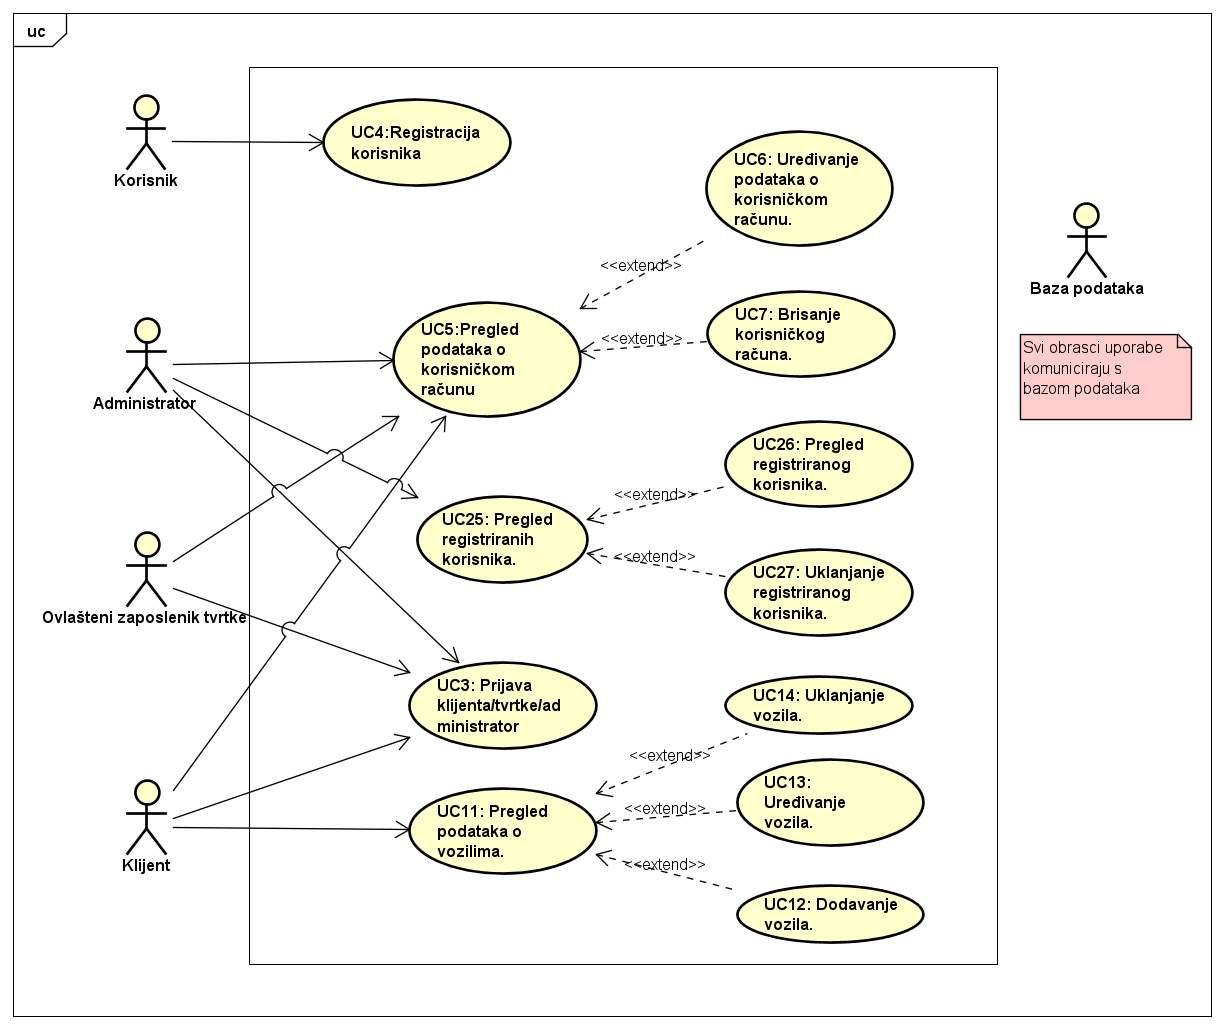
\includegraphics[width=1\linewidth]{dijagrami/Korisnički podaci.PNG} %veličina u odnosu na širinu linije
	\caption{Prikaz funkcionalnosti vezanih za korisničke podatke}
	\label{fig:promjene2} %label mora biti drugaciji za svaku sliku
\end{figure}
\begin{figure}[H]
	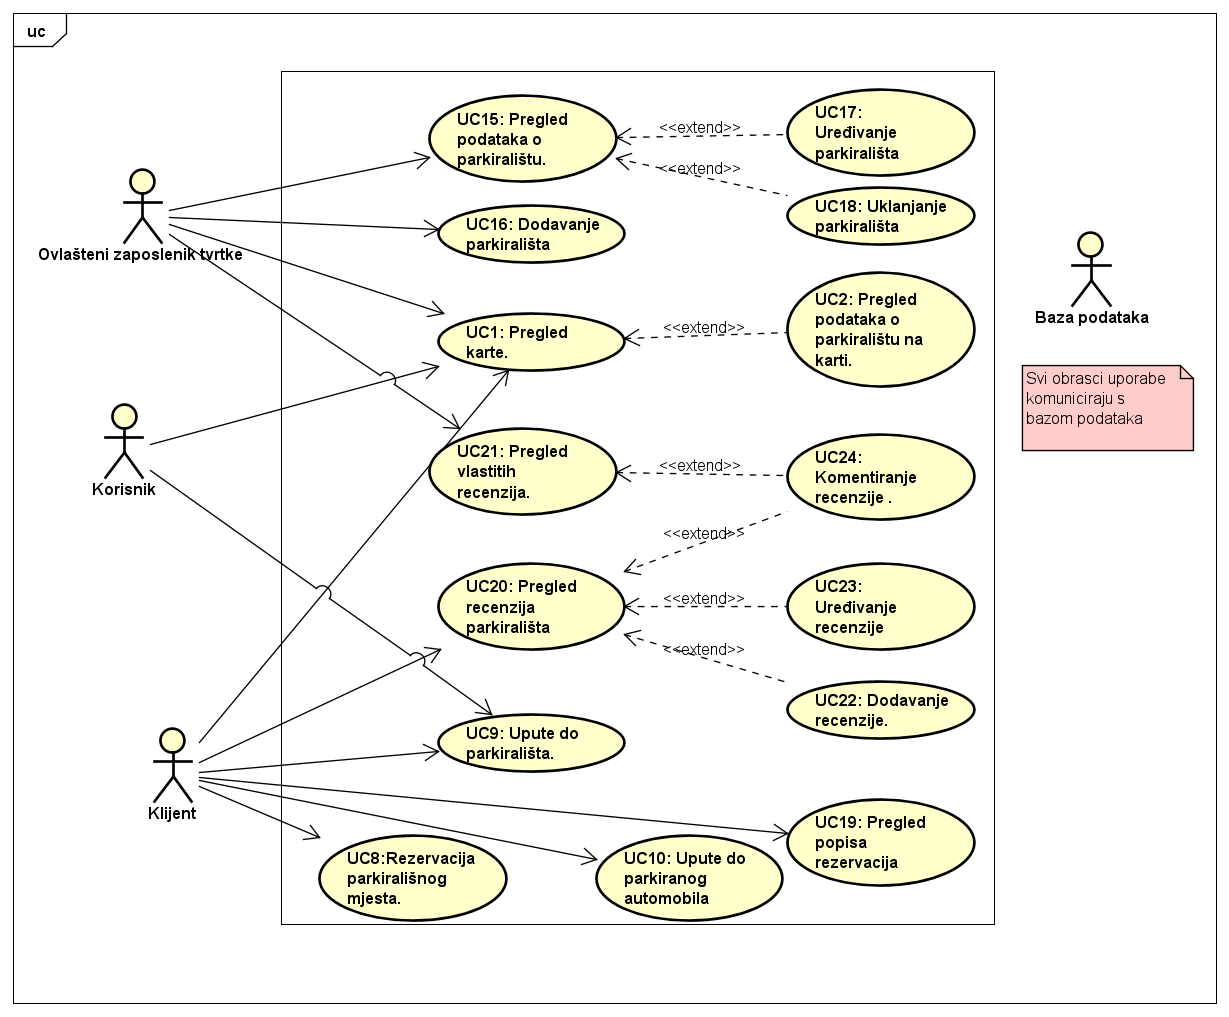
\includegraphics[width=1\linewidth]{dijagrami/Pregled ostalih funkcionalnosti.PNG} %veličina u odnosu na širinu linije
	\caption{Pregled ostalih funkcionalnosti}
	\label{fig:promjene2} %label mora biti drugaciji za svaku sliku
\end{figure}
\eject		

\subsection{Sekvencijski dijagrami}

\textbf{Obrazac uporabe UC4 - Registracija korisnika}\newline
Korisnik šalje zahtjev za registraciju. Poslužitelj prikazuje formu za popunjavanje korisničkih podataka. Korisnik unosi tražene podatke. U slučaju da neki od traženih podataka nisu validni (podatci nisu uneseni ili su uneseni neispravno) poslužitelj prikazuje odgovarajuću poruku za pojedini podatak korisnika.Ako su podatci validni, a nisu važeći (već postoji korisnik s istom e-mail adresom ili s istim OIB-om ????) poslužitelj prikazuje korisniku poruku o neuspjeloj registraciji. Ako su podatci važeći poslužitelj prikazuje poruku o uspješnoj registraciji te ga automatski prijavljuje u aplikaciju.\newline
\begin{figure}[H]
	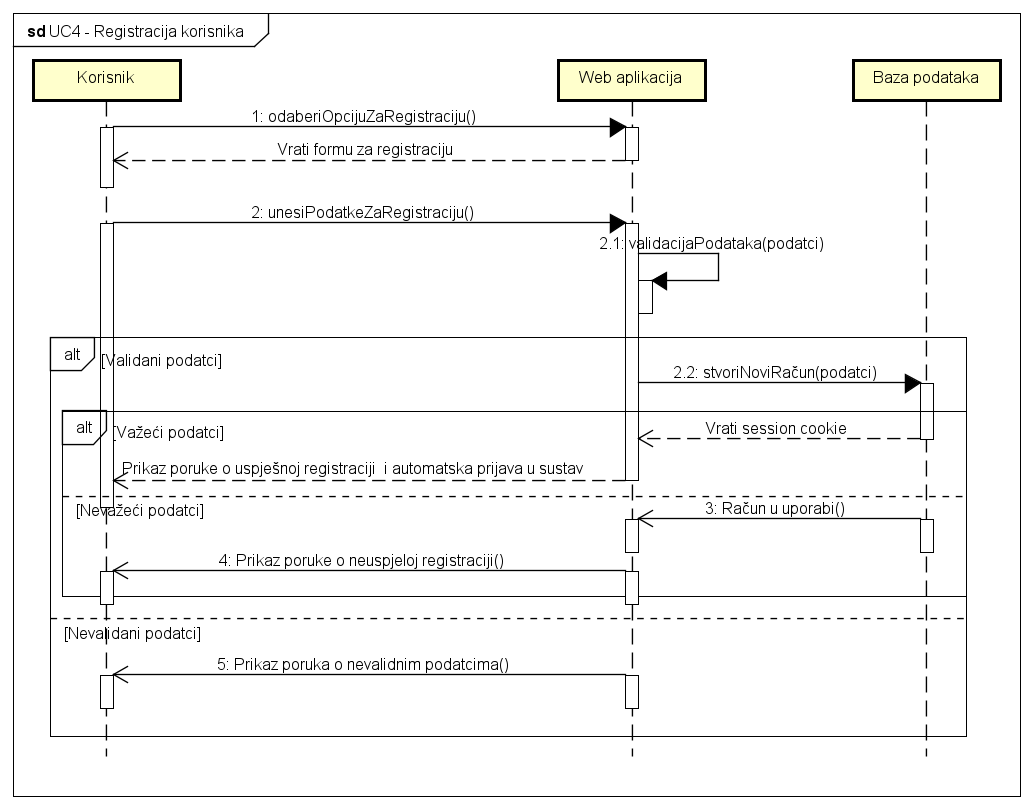
\includegraphics[width=1\linewidth]{dijagrami/UC4 - Registracija korisnika.png} %veličina u odnosu na širinu linije
	\caption{Sekvencijski dijagram za UC4}
	\label{fig:promjene2} %label mora biti drugaciji za svaku sliku
\end{figure}
\pagebreak
\textbf{Obrazac uporabe UC27 - Rezervacija parkirališnog mjesta}\newline
Klijent šalje zahtjev za prikaz karte s parkiralištima. Poslužitelj dohvaća i prikazuje prijavljena parkirališta. Odabirom parkirališta, poslužitelj iz baze podataka dohvaća osnovne podatke o parkiralištu i prikazuje ih korisniku. Kako bi obavio rezervaciju parkirališnog mjesta, klijent šalje zahtjev s tipom rezervacije i potrebne informacije vezane za rezervaciju. Poslužitelj provjerava ispravnost primljenih podatka o odabranoj rezervaciji te iz baze podataka dohvaća i provjera postoji li slobodno mjesto za traženi period na parkiralištu. Ukoliko nema slobodnih parkirališnih mjesta, sustav obavještava o tome klijenta. Ako postoji slobodno mjesto, proces rezervacije se nastavlja te se klijentu prikazuje sažetak rezervacije. Klijent tada potvrđuje plaćanje, ako kartica nema dovoljno sredstva na računu poslužitelj obavještava klijenta o neuspjelom plaćanju i vraća ga na prikaz karte. U slučaju da kartica ima dovoljno sredstva, sredstva se skidaju izravnim terećenjem. Rezervacija je završena i poslužitelj informaciju o rezervaciji prosljeđuje bazi koja sprema promjenu.\newline
\begin{figure}[H]
	\includegraphics[width=1\linewidth]{dijagrami/UC27-Rezervacija parkirališnog mjesta.png} %veličina u odnosu na širinu linije
	\caption{Sekvencijski dijagram za UC27}
	\label{fig:promjene2} %label mora biti drugaciji za svaku sliku
\end{figure}
\pagebreak
\textbf{Obrazac uporabe UC28 - Upute do parkirališta}\newline
Klijent šalje zahtjev za prikaz karte s parkiralištima. Poslužitelj dohvaća i prikazuje prijavljena parkirališta. Klijent odabire parkiralište do kojeg želi doći. Odabirom parkirališta, poslužitelj iz baze podataka dohvaća osnovne podatke o parkiralištu i prikazuje ih korisniku. Klijent šalje zahtjev za navigaciju do parkirališta. Poslužitelj otvara navigaciju te klijent dobiva upute kako doći do željenog parkirališta.
\begin{figure}[H]
	\includegraphics[width=1\linewidth]{dijagrami/UC28 - Upute do parkirališta.png} %veličina u odnosu na širinu linije
	\caption{Sekvencijski dijagram za UC28}
	\label{fig:promjene2} %label mora biti drugaciji za svaku sliku
\end{figure}
\eject

\section{Ostali zahtjevi}

\begin{packed_item}
	
	\item Sustav treba imati programsku potporu za web platformu s javnim sučeljem te prikazom karte s parkiralištima
	\item Sustav treba omogućavati istovremeni pristup za više korisnika 
	\item Programsko sučelje treba podržavati hrvatski jezik i dijakritičke znakove njegove abecede
	\item Sustav treba podržavati plaćanje u kunama
	\item Dohvat podataka iz baza mora se obaviti unutar nekoliko sekundi
	\item Sustav mora imati podršku za senzore koji očitavaju parkirna mjesta te komuniciraju s bazom podataka i redovito ju osvježavaju prilikom promjene stanja
    \item Sustav treba podržavati 3 vrste registracija:
        	\item[] \begin{packed_enum}
		
		\item Jednokratne rezervacije koje moraju biti napravljene barem 6 sati unaprijed te traju do 24 sata
		\item Ponavljajuće registracije koje moraju trajati barem 1 sat tjedno u razdoblju od minimalno mjesec dana
		\item Trajne rezervacije (0-24)
		
	\end{packed_enum}
    \item Sustav mora imati implementiranu podršku za oporavak u slučaju neispravnog korištenja korisničkog sučelja
    \item Sustav mora zabraniti pristup privatnim rutama. Ako korisnik nije bio prijavljen, preusmjerava se na formu za prijavu i ako nakon prijave ima ovlasti za tu rutu preusmjerava ga se na nju. Ako korisnik i dalje nema ovlasti ili nije bio prijavljen, preusmjerava ga se na početni zaslon aplikacije.
    \item Korisničko sučelje mora biti user friendly i jednostavno za korištenje
    \item Podaci koji se od korisnika prikupljaju i pohranjuju u bazu moraju biti zaštićeni i ograničenog pristupa
\end{packed_item}